\documentclass[12pt, oneside]{article}
\usepackage{a4wide}
\usepackage{oldgerm}
\usepackage{amsmath}
\usepackage{amssymb}
\usepackage{amstext}
\usepackage{graphicx}
\setlength{\textheight}{8.875in} \setlength{\textwidth}{6.875in}
\setlength{\columnsep}{0.3125in} \setlength{\topmargin}{0in}
\setlength{\headheight}{0in} \setlength{\headsep}{0in}
\setlength{\parindent}{1pc} \setlength{\oddsidemargin}{-.304in}
\setlength{\evensidemargin}{-.304in}



\begin{document}
\setlength{\textheight}{8.5in}
\centering {\bf MTL 390 (Statistical Methods) }\\


\centering{\bf Minor Examination Assignment 2 Report}



\vskip 0.5cm

\noindent Name: Hetvi Jethwani ~~~~~~~~~~~~~~~~~~~ Entry Number: 2018MT10754 ~~~~~~~~~~~~~~



\vskip 0.5cm


\begin{enumerate}

%--------------------------------------------

\item Testing of Hypothesis 
\newline Imagine working at a tele-communications company. Consider an exponential distribution to model the time in minutes till receiving of first phone call, with a rate of $\lambda$. Suppose $X_1,X_2,…,X_n$ are independent samples from this exponential distribution. Due to issues with clock precision, we don't have a very good resolution so we only have integral values of these samples- represented as $Y_1,Y_2,…,Y_n$. For example, if a particular sample corresponds to time 3.14 min we only have knowledge that it's 3 min owing to our clock.

\begin{enumerate}
    \item Consider a null hypothesis $H_0 : \lambda = \lambda_0$ with alternate hypothesis $H_1 : \lambda > \lambda_0$. $H_0$ is rejected if the sum of observed samples exceed a time $T_n$. Given a type-1 error $\alpha$, can you report $T_n$ such that the sequence of corresponding type-1 errors converges to $\alpha$?
    
    \item Your colleague presents a question to you, where they ask you to compare 2 independent random variables $Z_1 \sim Geo(p_1)$ and $Z_2 \sim Geo(p_2)$. Design an $\alpha$ test for $H_0 : p_1 = p_2$ against $H_1 : p_1 < p_2$.     

    \item Now, imagine we get access to a random sample $Z$ of a competitor company, which also models the time in minutes till receiving of first phone call using an exponential distribution. Similar to our predicament, they also get only integral values of these samples. Use parts (a) and (b) to design a test to compare our rate $\lambda$ with the competitor's rate $\lambda_c$.
\end{enumerate}

Answer:
\newline Part (a): We're given $[X_1],[X_2],...[X_n]$ where $[x]$ represents the integral part of $x$. The test is we have to reject $H_0$ if $\Sigma_{i=1}^{n} [X_i] > T_n$. 
\newline We're also given $X_i \sim Exp(\lambda)$. Note that $$P([X_i] = n) = P(n \le X_i < n+1) = e^{-n\lambda} - e^{-(n+1)\lambda} = (e^{-\lambda})^n (1-e^{\lambda})$$
So, for $p = 1 - e^{\lambda}$, $[X_i] \sim Geom(p)$. Now, we'll prove that $\Sigma_{i=1}^{n} [X_i] \sim NegativeBinomial(n,p)$ by induction.
\newline Base case: for $Y_1,Y_2 \sim Geom(p)$, both are independent. 
$$P(Y_1 + Y_2 = y) = \Sigma_{i=0}^{y} P(Y_1 = i) P(Y_2 = y-i) = \Sigma_{i=0}^{y} p(1-p)^i p (1-p)^{y-i}$$
So, 
$$P(Y_1 + Y_2 = y) = {2+y-1 \choose y} p^2 (1-p)^{y} \implies Y_1 + Y_2 \sim NegativeBinomial(2,p)$$
\newline Inductive step: For $Y_i \sim Geom(p), i=1,2,...k$ we have $\Sigma_{i=1}^{k-1} Y_i \sim NegativeBinomial(k-1,p)$. We will prove that $\Sigma_{i=1}^{k} Y_i \sim NegativeBinomial(k,p)$. We have,

$$P(\Sigma_{i=1}^{k-1} Y_i + Y_{k} = y) = \Sigma_{i=0}^{y} P(\Sigma_{i=1}^{k-1} Y_i = i) P(Y_k = y-i) \text{   since $Y_i's$ independent}$$
Or,
$$ = \Sigma_{i=0}^{y} {k-1+i-1 \choose i} p^{k-1} (1-p)^i p (1-p)^{y-i} = p^k (1-p)^y \Sigma_{i=0}^{y} {k+i-2 \choose i}$$
Thus,
$$P(\Sigma_{i=1}^{k} Y_i = y) = {k+y-1 \choose y} p^k (1-p)^y \implies \Sigma_{i=1}^{k} Y_i = y \sim NegativeBinomial(k,p)$$. 

Let mean of $NegativeBinomial(k,p)$ is represented by $\mu_k,$ standard deviation represented by $\sigma_k$. Here,
$$\mu_k = k E([X_1]) = \dfrac{k(1-p)}{p}$$ and by Bienaymé formula, 
$Var(\Sigma_{i=1}^{k} Y_i) = \Sigma_{i=1}^{k} var(Y_i)$ so
$$\sigma_k = \sqrt{\dfrac{k(1-p)}{p^2}}$$
 
Thus, we can conclude that $\Sigma_{i=1}^{n} [X_i] \sim NegativeBinomial(n,p)$ where $p = 1 - e^{-\lambda}$. Here, let $\Sigma_{i=1}^{n} [X_i] = S_n$ and $\alpha_n$ be the type-1 error for the given $H_0$ and $H_1,$ we have

$$\alpha_n = P(S_n > T_n | \lambda = \lambda_0)$$

As $n \to \infty, \dfrac{S_n -\mu_n}{\sigma_n/ \sqrt{n}} \to N(0,1)$, by confidence intervals for the standard normal distribution, we have 
$$
\dfrac{T_n -\mu_n}{\sigma_n/ \sqrt{n}} = Z_{\alpha} \implies T_n = \dfrac{Z_{\alpha} \sigma_n}{\sqrt{n}} + \mu_n = \dfrac{Z_{\alpha} \sqrt{1-p} + n(1-p)}{p}
$$, where $p = 1 - e^{-\lambda}$.
\newline Part (b): We have $Z_1,Z_2$ independent geometrically distributed random variables. From part (a), we know that for $Y = Z_1 + Z_2, Y \sim NegativeBinomial(2,p)$ if $p_1=p_2=p$. 
Note that if $p_1=p_2=p$, $$P(Z_1 = z_1 | Y = y) = \dfrac{P(Z_2 = y - z_1)P(Z_1 = z_1)}{P(Y=y)} = \dfrac{1}{y+1}.$$
Now, $$
P_{H_0}(Z_1 > c | Y = y) = \dfrac{y-c}{y+1} = \alpha \implies c = (1-\alpha)y - \alpha
$$. 
So we design test, reject $H_0$ if given values $z_1,z_2$ were observed, $z_1 > (1-\alpha)(z_1 + z_2) - \alpha,$ or equivalently if $z_1 > \dfrac{(1-\alpha)z_2}{\alpha}-1$.
\newline Part (c): We have $[X_1] \sim Geom(1-e^{\lambda}),$ and $[Z_1] \sim Geom(1-e^{-\lambda_c})$. Proceed using part (b). Note that 
$p_1 = p_2 \iff \lambda = \lambda_c$ and $p_1 < p_2 \iff \lambda_c > \lambda$ so the equivalent hypotheses are $H_0: \lambda = \lambda_c$ and $H_1 : \lambda_c > \lambda$.

\item Testing of Hypothesis 
\begin{enumerate}
    \item Alice and Bob have access to different samples each from the same coin-toss experiment, $S_a = \{ A_1, A_2,...A_n \}$ and $S_b = \{ B_1,B_2,...B_m \}$ respectively. The hypothesis $H_0: \textit{coin is unbiased}$ is to be tested. If they combine their sample spaces, how does that affect the power of any given test? 
    \item In part (a), consider $H_1 : \textit{H is expected to occur less frequently than T}$ and design the uniformly most powerful test for $S_a, S_b, S_a \cup S_b$ of significance $\alpha$. % Use it to validate that part (a) holds by taking an example of your choice.

    \item Now, Carol comes and gives Alice and Bob new iid generated samples- $C_1, C_2, ...C_n$. She tells them to test if these were obtained from $H_0: \textit{toss of a fair coin}$ or $H_1 : \textit{from a mixed experiment defined as follows.}$ 
    \newline Experiment: Toss a fair coin, if it's heads then generate $C_i's$ from a coin which gives heads $75\%$ of the time, else generate $C_i's$ from a coin which gives tails $75\%$ of the time. Rationalize why a threshold test on likelihood ratio will work.  
    
    % \item Alice, Bob, and Carol get talking about a statistical thought experiment- where they have an oracle which measures if Mt. Etna just exploded or not. The oracle, internally, has a fair slot machine which outputs a number from $1$ to $8$. It queries this machine twice and lies if the sum of both observations is more than $14$. Alice says, "the probability of this happening by chance is 2/64, since the level of significance is less than 0.05, we conclude that Mt. Etna exploded." Is her statement correct? Can you help her be more precise? 
    \item The friends begin talking about their own research, where Carol, a biologist, and also editor at a prestigious journal mentions their policy of publishing papers about medical treatments only if the conclusion about their effectiveness/ineffectiveness holds at the 95\% confidence level, even checking for similar treatments whose control studies were done independently. She proudly states that they can be confident that at most 1 out of the 20 independent studies they published in the past year was a mistake- since the probability of making a mistake is $(0.05)^{20}$, which is negligible. But Alice and Bob disagree with her and claim that it's possible for all 20 studies to be wrong too- help them explain the flaw in her reasoning. 
    
% https://xkcd.com/1132/

\end{enumerate}
Answer:
\newline Part (a): The power is the likelihood that our test will distinguish an effect of a certain size from pure luck. More number of samples will lead to a lower $\beta,$ since 

$$\beta = P(X_n \in \text{Acceptance region} | H_0 \text{ false})$$

and note that as $n$ gets large, the acceptance region gets smaller and closer to the value of the null hypothesis. Thus, we expect power to increase, since it is given by $1-\beta.$ Intuitively, larger the number of samples- the more data we have to separate some significant pattern from random variation. 
\newline Part (b): Consider a general set of i.i.d. samples $X_1,X_2,...X_k \sim Bernoulli(p)$ where $x_i = 1 \implies \text{coin showed heads}$ and it shows heads with probability $p$. It's given that 
$$H_0 : p = 0.5; H_1 : p < 0.5$$
The likelihood under $H_0$ is $$
f_0(x) = \Pi_{i=1}^{k} 0.5 = 0.5^k 
$$
The likelihood under $H_1$ is $$f_1(x) = \Pi_{i=1}^{k} p^{x_i} (1-p)^{1-x_i}= (1-p)^{k} (\dfrac{p}{1-p})^{x_1+...+x_k}$$.
Thus, likelihood ratio can be given as 

$$\dfrac{f_0}{f_1} = \dfrac{1}{(2(1-p))^k} (\dfrac{1-p}{p})^{x_1+...+x_k}$$. 
Note that $$p < 0.5 \implies \frac{1}{p} > 2 \implies \frac{1-p}{p} > 1.$$ 
As $\Sigma_{i=1}^{k} x_i$ increases, $\dfrac{f_0}{f_1}$ increases. By Neyman-Pearson lemma, we can say that the most powerful test will be such that null is rejected if $\Sigma_{i=1}^{k} X_i < c$ for some $c$.

Now, $X_i \sim Bernoulli(p) \implies \Sigma_{i=1}^{k} X_i \sim Binomial(n,p)$. To maintain significance $\alpha,$ we'll have 

$$\alpha = P(\Sigma_{i=1}^{k} X_i < c | \Sigma_{i=1}^{k} X_i \sim Binomial(k,0.5))$$
Or, $c$ is given by the $\alpha$ quantile of distribution $Binomial(k,0.5)$. Since $c$ doesn't depend on $p$, the most powerful test is also uniformly most powerful. 
\newline For $S_a,$ the coin is fair if $\Sigma_{i=1}^{n} A_i < c_a$. For $S_b,$ the coin is fair if $\Sigma_{i=1}^{m} B_i < c_b$. For $S_a \cup S_b,$ the coin is fair if $\Sigma_{i=1}^{n} A_i + \Sigma_{i=1}^{m} B_i < c_{ab}$ where $c_a$ is $\alpha$ quantile of $Binomial(n,0.5)$, $c_b$ is $\alpha$ quantile of $Binomial(m,0.5)$ and $c_{ab}$ is $\alpha$ quantile of $Binomial(n+m,0.5)$ respectively. 

Part (c): For iid generated samples $C_1,...C_n$ it's given that 
$$H_0 : C_i \sim Bernoulli(0.5); H_1 : C_i \sim Experiment.$$ 
Let $S_n = \Sigma_{i=1}^{n} C_i$

The likelihood under $H_0$ is $$
f_0(x) = \Pi_{i=1}^{n} 0.5 = 0.5^n 
$$
The likelihood under $H_1$ is $$f_1(x) = 0.5(\Pi_{i=1}^{n} p^{c_i} (1-p)^{1-c_i} + \Pi_{i=1}^{n} p^{1-c_i} (1-p)^{c_i}) = 0.5((1-p)^n (\dfrac{p}{1-p})^{s_n} + (p)^n (\dfrac{1-p}{p})^{s_n})$$
Since $p = 0.75,$
$$f_1 = \dfrac{3^{s_n} + 3^{n-s_n}}{2*4^n}
$$
Thus, likelihood ratio can be given as 

$$\dfrac{f_0}{f_1} = \dfrac{2^{n+1}}{3^{s_n} + 3^{n-s_n}}.$$ 
This will work because, essentially putting a threshold on the ratio for a given value of n means putting a threshold on $3^{s_n} + 3^{n-s_n}$. 
For sufficiently large $n,$ under $H_0$ we have $3^{s_n} + 3^{n-s_n} \approx 2*3^{0.5n} = (\dfrac{\sqrt{3}}{2})^n$. This will go to $0$ as $n \to \infty$.    

Under $H_1$ we have $3^{s_n} + 3^{n-s_n} \approx 3^{0.25n} + 3^{0.75n} = (3^{0.25})^n + (27^{0.25})^n$ but here $(27^{0.25})^n \to \infty$ as $n \to \infty$ so this value will be very large and increase with $n$. Thus, the test will work due to these cases being clearly distinguishable by putting a suitable threshold on the likelihood ratio. The value of the threshold would depend on required significance level. 

Part (d): Carol has confused the statistical confidence level with probability. A treatment is either effective or not in absolution in real life, we're using a statistical experiment to try and model its efficacy, namely by conducting many, many trials of the treatment. A confidence level of 95\% means that reasonably, 95\% of \textbf{all conducted} trials would yield a correct conclusion. But in a real life setting- not all trials are submitted for publication. For example, if a scientist conducts $500$ trials of a treatment which is ineffective (but it's not known) then $500/20 = 25$ trials will look helpful even when they aren't, and the remaining 475 trials wouldn't be submitted for publication since they didn't show positive results at the confidence level, hence resulting in a honestly done but 'misleading' publication. 

% Part (d): Alice is correct in saying that the event occurs with probability $3/64 \approx 0.046$. Note that here the conditional probability being talked about P(Etna explodes $| H_0$ true) but the p value is the probability of getting a test statistic as extreme or more extreme than the calculated test statistic. The test statistic is something we define to validate or reject our hypotheses. \newline A better way to talk about significance here is using the rejection region.


% -------
\item Testing of Hypothesis 
\begin{enumerate}
    \item Dave is struggling to apply the Neyman-Pearson lemma on continuous distributions. Help him find the uniformly most powerful test for the case of $n$ samples drawn from a normal population $N(\mu,1)$, testing $H_0:\mu = \mu_0,$ against $H_1: \mu > \mu_0$ and $H_1: \mu < \mu_0$. Interpret this geometrically for $n=2$, clearly highlighting critical region. Use the graph to highlight why we can't have UMP test for $H_1 : \mu \neq \mu_0$. He starts wondering what happens when $n$ samples are instead drawn from a normal population $N(0,\sigma)$ and test $H_0: \sigma = \sigma_0$ against $H_1: \sigma > \sigma_1$ and $H_1: \sigma < \sigma_1$. Find the most powerful test for various cases, and interpret it geometrically for $n=2$, clearly highlighting critical region. Can we design a uniformly most powerful test in this case?

    \item Equipped with his newfound interest in statistics, Dave designs an experiment to deal with severity of symptoms post-vaccination. He asks people who have gotten only the first shot of 3 different kinds of COVID vaccines about their experiences, and asks them to give a number on a $0-4$ scale about the severity of discomfort they experienced $24-48$ hrs after getting vaccinated. He collects data as follows- 

    \begin{table}[!ht]
    \centering
    \begin{tabular}{|l|l|l|l|}
    \hline
    Vaccine:        & Covishield & Covaxin & Moderna  \\ \hline
    Sample $\mu$    & 1      & 0.7     & 1.3      \\ \hline
    Sample $\sigma$ & 1.054     & 0.9487  & 0.8233    \\ \hline
    Sample size     & 10         & 10      & 10         \\ \hline
    \end{tabular}
    \end{table}
    Are the mean severity effects of these vaccines distinguishable? Can one vaccine be advised over another? Help him answer using one-sided ANOVA test.

    \item Dave's friend, Eve comes and gives Dave 10 samples she took from people who got the same brand of vaccine- but she doesn't know which vaccine they got. 
    \begin{table}[!htb]
    \centering
    \begin{tabular}{|l|l|l|l|l|l|l|l|l|l|l|}
    \hline
    Dave & 0 & 3 & 0 & 0 & 1 & 1 & 0 & 1 & 1 & 0 \\ \hline
    Eve  & 0 & 0 & 0 & 1 & 1 & 1 & x & 2 & 3 & 3 \\ \hline
    \end{tabular}
    \end{table}
    On applying median test to this data at level of significance 85\% and comparing it to covaxin data collected by Dave, Eve remembers getting a statistically significant result. What are the possible values of $x$? [In case of equality with median, count as 'below' median].
    
\end{enumerate}
Answer:
\newline Part (a): First, let's find the most powerful test for when $H_1: \mu = \mu_1$, for cases when $\mu_1 > \mu_0$ and $\mu_1 < \mu_0$.
\newline The likelihood ratio is 
$$
\dfrac{f_1}{f_0} = \dfrac{exp[-0.5\Sigma_{i=1}^{n} (x_i-\mu_1)^2]}{exp[-0.5\Sigma_{i=1}^{n} (x_i-\mu_0)^2]} = exp[-0.5\Sigma_{i=1}^{n} [(x_i-\mu_1)^2 - (x_i-\mu_0)^2]]
$$
So, $$
\dfrac{f_1}{f_0} \ge k \implies -0.5\Sigma_{i=1}^{n} [(x_i-\mu_1)^2 - (x_i-\mu_0)^2] \ge log(k) 
$$
Or, 
$$-0.5n(\mu_1^2 - \mu_0^2) + (\mu_1 - \mu_0) (\Sigma_{i=1}^{n} x_i) \ge log(k)$$
Or,
$$ (\mu_1 - \mu_0) \bar{x} \ge log(k)/n + 0.5(\mu_1^2 - \mu_0^2).$$

Case 1: $\mu_1 > \mu_0$
$$
\bar{x} \ge \dfrac{log(k)}{n(\mu_1 - \mu_0)} + 0.5(\mu_1 + \mu_0)
$$
Let $\dfrac{log(k)}{n(\mu_1 - \mu_0)} + 0.5(\mu_1 + \mu_0) = c_1$, it is given by
$\alpha = P(\bar{x} > c_1 | H_0),$ so
$$
c_1 = \mu_0 + \dfrac{Z_{\alpha}}{\sqrt{n}}.$$
Since $c_1$ doesn't change with $\mu_1,$ it is a UMP test. 
For $n=2,$ we reject $H_0$ if $x_1 + x_2 > 2c_1$. 

Case 1: $\mu_1 < \mu_0$
$$
\bar{x} < \dfrac{log(k)}{n(\mu_1 - \mu_0)} + 0.5(\mu_1 + \mu_0)
$$
Let $\dfrac{log(k)}{n(\mu_1 - \mu_0)} + 0.5(\mu_1 + \mu_0) = c_2$, it is given by
$\alpha = P(\bar{x} < c_2 | H_0),$ so
$$
c_2 = \mu_0 + \dfrac{Z_{1-\alpha}}{\sqrt{n}} = \mu_0 - \dfrac{Z_{\alpha}}{\sqrt{n}}.$$
Since $c_2$ doesn't change with $\mu_1,$ it is a UMP test. 
For $n=2,$ we reject $H_0$ if $x_1 + x_2 < 2c_2$. 
The visualization is shown in Figure \ref{fig:q3}. 
We can't have a UMP for case where $H_1 : \mu \neq \mu_0$ because the critical regions for $\mu > \mu_0$ and $\mu < \mu_0$ are disjoint. 

\begin{figure}[!ht]
    \centering
    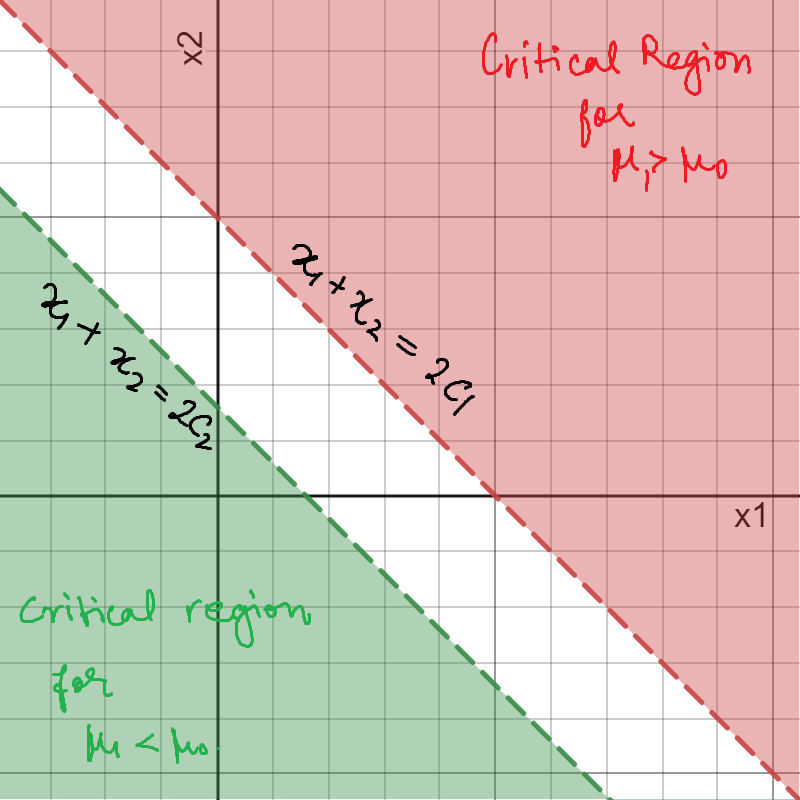
\includegraphics[width=0.6\textwidth]{desmos-graph.png}
    \caption{\label{fig:q3} For Q3. Part (a)}
\end{figure}

For the next case, we'll have the likelihood ratio as 
$$
\dfrac{f_1}{f_0} = \dfrac{exp[-(0.5/\sigma_1^2)\Sigma_{i=1}^{n} (x_i)^2]}{exp[-(0.5/\sigma_0^2)\Sigma_{i=1}^{n} (x_i)^2]} = exp[-0.5\Sigma_{i=1}^{n}(x_i^2) [1/(\sigma_1^2)-1/(\sigma_0^2)]]
$$
So,
$$
\dfrac{f_1}{f_0} \ge k \implies \Sigma_{i=1}^{n} x_i^2 \ge \dfrac{2log(k)\sigma_1^2\sigma_0^2}{\sigma_1^2 - \sigma_0^2} 
$$
Now $c$ is determined according to $\alpha$ as 
\newline Against $H_1: \sigma_1 > \sigma_0$, let $c = \dfrac{2log(k)\sigma_1^2\sigma_0^2}{\sigma_1^2 - \sigma_0^2}$,
$$
P(\Sigma_{i=1}^{n} x_i^2 \ge c | H_0) = \alpha \implies P(\Sigma_{i=1}^{n} (x_i/\sigma_0)^2 \le c/(\sigma_0^2) | H_0) = 1-\alpha
$$
$$
\implies c = \sigma_0^2 \chi_{1-\alpha,n}^2
$$

Against $H_1: \sigma_1 < \sigma_0$, let $c = \dfrac{2log(k)\sigma_1^2\sigma_0^2}{\sigma_0^2 - \sigma_1^2}$,
$$
P(\Sigma_{i=1}^{n} x_i^2 \le c | H_0) = \alpha \implies \implies c = \sigma_0^2 \chi_{\alpha,n}^2
$$

Thus, for $H_1: \sigma_0 \neq \sigma_1$ our critical region will be $\{ 
\Sigma_{i=1}^{n} x_i^2 \ge \sigma_0^2 \chi_{1-\alpha,n}^2 \} \cup \{ 
\Sigma_{i=1}^{n} x_i^2 \le \sigma_0^2 \chi_{\alpha,n}^2\}$. 


We can't have a UMP for case where $H_1 : \mu \neq \mu_0$ because the critical regions for $\mu > \mu_0$ and $\mu < \mu_0$ are disjoint. For $n=2,$ plotting the critical region-


\begin{figure}[!ht]
    \centering
    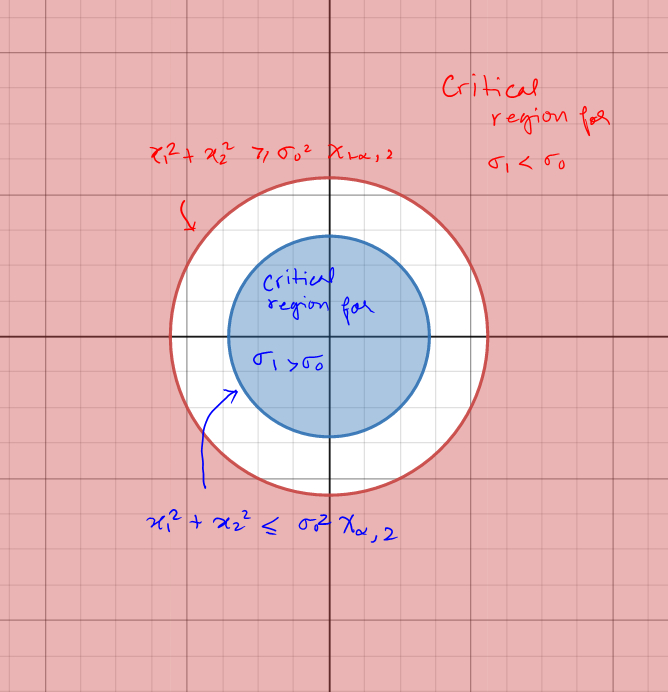
\includegraphics[width=0.6\textwidth]{390_asst_q3parta_2.PNG}
    \caption{\label{fig:q3} For Q3. Part (a)}
\end{figure}


Part (b): Applying ANOVA. 
\newline Recall that 
$$
H_0 : \mu_1 = \mu_2 = \mu_3; H_1 : \text{At least one pair of sample means is significantly different}
$$
\newline Grand mean is 1, so $\bar{x_G} = 1$. 
$$SS_b = 10 \Sigma_{i=1}^{3} (\bar{x_i} - \bar{x_G})^2 = 1.8$$

$$SS_w = \Sigma_{i=1}^{3} \Sigma_{j=1}^{10} (x_{ij} - \bar{x_i})^2 = 24.2008$$

We build the ANOVA table as follows-
\begin{table}[!ht]
\centering
\begin{tabular}{|l|l|l|l|}
\hline
$SS_b = 1.8$ & $df_b = 2$ & $MS_b = 0.9$ & $F_0 = \dfrac{MS_b}{MS_w}$ \\ \hline
$SS_w = 24.2008$ & $df_w = 27$ & $MS_w = 0.8963$ & $F_0 = 1.0041$                   \\ \hline
\end{tabular}
\end{table}
Now, $F_{k-1,N-k,\alpha} = F_{2,27,0.1} = 2.5106$ thus, $H_0$ is accepted and we conclude that there's no statistical significance in the mean-severity of each vaccine. Thus, any vaccine should be taken. 
\newline Part (c): For grand median- we don't know where $x$ is so we'll have to make cases since there are 8 zeroes in combined sample space. If $x = 0, M = 0.5$ else $x > 0, M = 1$. Further, we'll have to make a case distinguishing value of x at 1 with x > 1 since the median test counting will change. The test statistic here is $\chi^2 = \dfrac{N(ad-bc)^2}{(a+b)(a+c)(b+d)(c+d)}$. 

Case 1: $x = 0 \implies M =0.5$.
\begin{table}[!ht]
\centering
\begin{tabular}{|l|l|l|l|}
\hline
               & Dave & Eve & row-sum          \\ \hline
\textgreater M & 5    & 6   & 11               \\ \hline
$\le$ M        & 5    & 4   & 9                \\ \hline
col-sum        & 10   & 10  & $\chi^2 = 0.202$ \\ \hline
\end{tabular}
\end{table}

Case 2: $x = 1$
\begin{table}[!ht]
\centering
\begin{tabular}{|l|l|l|l|}
\hline
               & Dave & Eve & row-sum          \\ \hline
\textgreater M & 1    & 3   & 4               \\ \hline
$\le$ M        & 9    & 7   & 16                \\ \hline
col-sum        & 10   & 10  & $\chi^2 = 1.25$ \\ \hline
\end{tabular}
\end{table}

Case 3: $x > 1$
\begin{table}[!ht]
\centering
\begin{tabular}{|l|l|l|l|}
\hline
               & Dave & Eve & row-sum          \\ \hline
\textgreater M & 1   & 4  & 5               \\ \hline
$\le$ M        & 9    & 6   & 15                \\ \hline
col-sum        & 10   & 10  & $\chi^2 = 2.4$ \\ \hline
\end{tabular}
\end{table}

For $\alpha = 0.15, \chi^2_{1,\alpha} = 2.072$ so $x = 0$ or $x = 1$.

\item Analysis of correlation and regression
\begin{enumerate}
    \item The coefficient of rank correlation of points scored by 10 dogs in 2 different events (out of a total of 10 points) at a pet-show was found to be 0.5, but it was realized that one of the dogs was wrongly marked as 8 and 5 instead of 8 and $x$ in the 2 events. The corrected rank coefficient was found as $0.2576$. What was the true score of the dog?
    
    \item If the regression of $Y$ on $X$ is linear, is it necessary for the regression of $X$ on $Y$ to be linear? 
    
    \item Given samples $(X_1,Y_1),....(X_n,Y_n)$, find the angle between the line of regression of $Y$ on $X$ and $X$ on $Y$. Use this to comment on the correlation between $X$ and $Y$ in the following plots. 
    \begin{figure}[!ht]
        \centering
        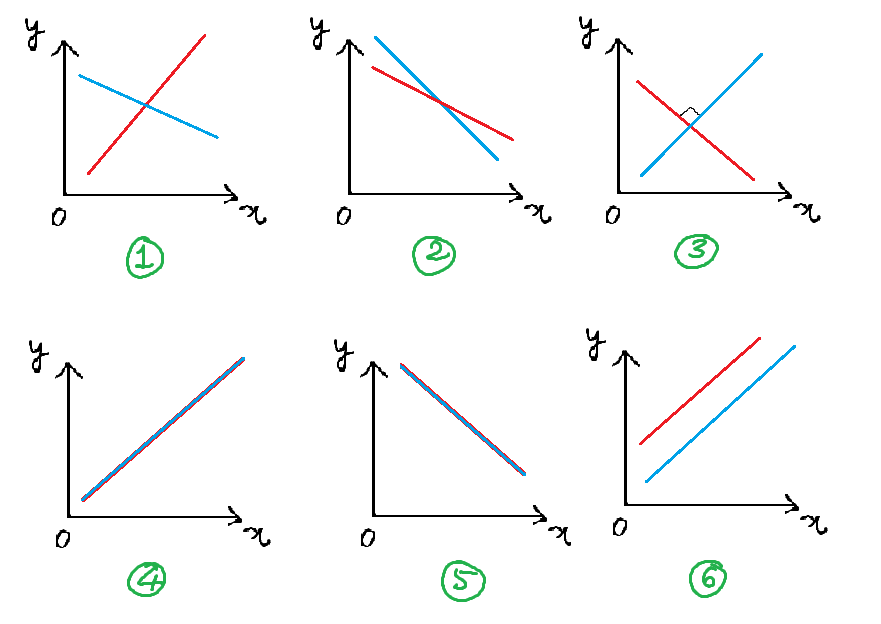
\includegraphics[width=\textwidth]{coorrplots.png}
        \caption{\label{fig:cp} For Q4 (c)}
    \end{figure}
    
    \item 3 different groups of professionals were asked if the status of the current healthcare system was worse, the same or better than one year ago. Is there a correlation between their opinion and their profession?
    \begin{table}[!htb]
    \centering
\begin{tabular}{|l|lll|l|}
\hline
               & \multicolumn{1}{l|}{Worse} & \multicolumn{1}{l|}{Same} & Better &     \\ \hline
Doctors        & 20                         & 15                        & 12     & 47  \\ \cline{1-1} \cline{5-5} 
Administrators & 24                         & 27                        & 32     & 83  \\ \cline{1-1} \cline{5-5} 
Artists        & 14                         & 22                        & 23     & 59  \\ \hline
               & \multicolumn{1}{l|}{58}    & \multicolumn{1}{l|}{64}   & 67     & 189 \\ \hline
\end{tabular}
\end{table}
\end{enumerate}


Answer:
\newline Part (a): Let difference of ranks be $D$ with first set of observations.
\newline Old correlation coefficient,
$$
0.5 = 1 - \dfrac{6D}{990} \implies D = 990/12 = 82.5
$$
On correcting,
$$
D' = D - 3^2 + (8-x)^2 = 73.5 + (8-x)^2
$$
So, corrected correlation coefficient,
$$
0.2576 = 1 - \dfrac{6D'}{990} \implies 73.5 + (8-x)^2 = 165*0.7424 \implies 
(8-x) = \pm 7$$
Thus, $x = 1$ since points can't exceed 10 for each event.
\newline Part (b): Not necessary. Consider 
$f(x,y) = 1$ when $|y| < x, x \in (0,1)$ and
$f(x,y) = 0$ otherwise. 

$$
f_x = \int_{-x}^{x} f(x,y) dy = \int_{-x}^{x} 1 dy = 2x, x \in (0,1)
$$

$$
f_y = \int_{|y|}^{1} f(x,y) dx = \int_{|y|}^{1} 1 dx = 1 - |y|, y \in (-1,1)
$$

$$
E(Y|X) = \int_{-x}^{x} y \dfrac{f(x,y)}{f_x} dy = \int_{-x}^{x} y/2x dy = 0
$$

$$
\text{For y $\in (0,1)$, } 
E(X|Y=y) = \int_{0}^{1} x \dfrac{f(x,y)}{f_y} dx = \int_{0}^{1} \dfrac{x}{1-y} dx = \dfrac{1}{2(1-y)} 
$$

$$
\text{For y $\in (-1,0)$, } 
E(X|Y=y) = \int_{0}^{1} x \dfrac{f(x,y)}{f_y} dx = \int_{0}^{1} \dfrac{x}{1+y} dx = \dfrac{1}{2(1+y)} 
$$
Clearly, $E(X|Y)$ isn't linear but $E(Y|X)$ is.
\newline Part (c): We know that line of regression of $Y$ on $X$ is given by $\hat{y} - \bar{y} = \dfrac{S_{xy}}{S_{xx}}(x - \bar{x})$. Line of regression of $X$ on $Y$ is thus given as, $\hat{x} - \bar{x} = \dfrac{S_{yx}}{S_{yy}}(y - \bar{y}) \implies y - \bar{y} = \dfrac{S_{yy}}{S_{xy}}(\hat{x} - \bar{x})$. The angle between them is
$$
tan \theta = \dfrac{S_{yy}/S_{xy} - S_{xy}/S_{xx}}{1 + S_{yy}/S_{xx}} = \dfrac{1-r^2}{r} \dfrac{\sqrt{S_{xx}S_{yy}}}{S_{xx}+S_{yy}}
$$
where $r$ is correlation coefficient. A rough 2D plot of $\theta v/s r$ will help us answer the following questions. 
\begin{figure}[!ht]
    \centering
    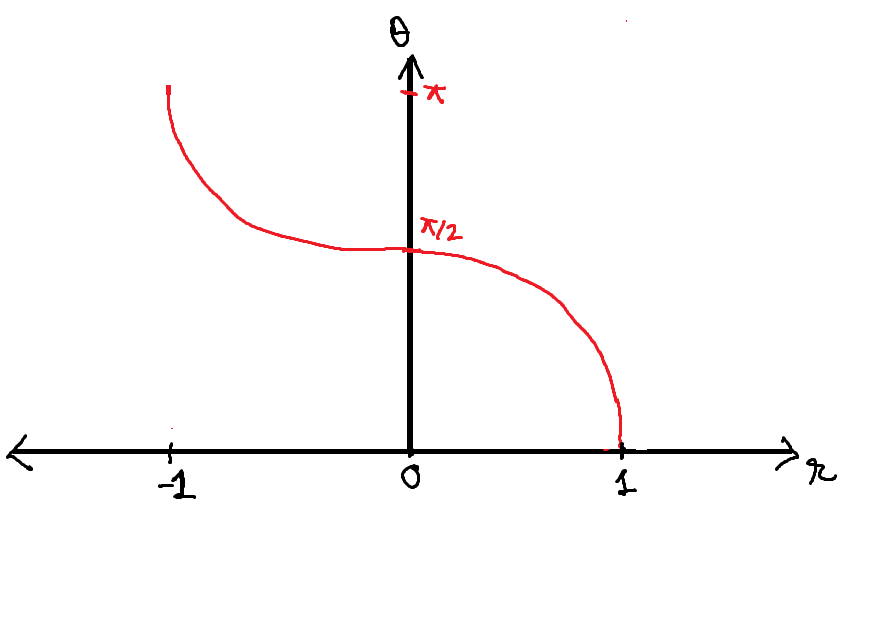
\includegraphics[width=0.5\textwidth]{roughthetar.png}
    \caption{\label{fig:rtr} Rough sketch of $\theta$ v/s r}
\end{figure}

Thus, for the given plots, 1 is low correlation, and 2 is high correlation, 3 is uncorrelated, 4 is correlation with $r=1$, 5 is correlation with $r=-1$ and 6 isn't possible since if the lines aren't intersecting then they're parallel but here, being parallel implies they must coincide by properties of $r$. 

Part (d): The chi-squared statistic here is 
$$
\dfrac{(20-47*58/189)}{47*58/189} + \dfrac{(15-47*64/189)}{47*64/189} + ... + \dfrac{(23-67*59/189)}{67*59/189}  \approx 5.2
$$
To be tested against $\chi^2_{0.05,(3-1)(3-1)} \approx 9.5$
Since $5.21 < 9.5 \implies$ the null hypothesis that they're independent is accepted, thus opinion and profession aren't correlated. 

\item Analysis of correlation and regression

\begin{enumerate}
    \item $X,Y$ are standardized random variables, and $r(aX+bY,aY+bX) = \dfrac{1+2ab}{a^2+b^2}$. What's the correlation coefficient between $X$ and $Y$?
    \item Ferb calculates the estimated linear regression equations of $Y$ on $X$ and $X$ on $Y$ as $8X + 10Y + 66 = 0$ and $40X - 18Y = 214$ respectively. What is the fallacy here? He realizes the fallacy and corrects the equations to be $8X - 10Y + 66 = 0$ and $40X - 18Y = 214$ respectively- but there's another fallacy here! What's the fallacy?
    \item Ferb thinks that if $X_1 = aX_2 + c$ and $X_1 = bX_3 + d$ then the multiple regression would have partial slopes identical to $a,b$ for $X_2,X_3$ respectively. Prove him wrong by using the following table, take $n=102$. For each equation, which coefficients are statistically significant? What's $R^2$ and adjusted $R^2$? 
    \begin{table}[!ht]
    \centering
    \begin{tabular}{|l|l|l|l|}
    \hline
          & Mean  & Std. Deviation & Partial correlation \\ \hline
    $X_1$ & 28.02 & 4.42           & $r_{12} = 0.80$     \\ \hline
    $X_2$ & 4.91  & 1.10           & $r_{23} = -0.56$    \\ \hline
    $X_3$ & 594   & 85             & $r_{31} = -0.40$    \\ \hline
    \end{tabular}
    \end{table}
\end{enumerate}
\item 

Answer:
\newline Part (a): Given: $E(X) = E(Y) = 0, Var(X) = Var(Y) = 1 \implies E(X^2) = E(Y^2) = 1,$ and $r(X,Y) = E(XY) - E(X)E(Y) = E(XY).$
$$
r(aX+bY, aY+bX) = \dfrac{E((aX+bY)(aY+bX))-E(aX+bY)E( aY+bX)}{\sqrt{Var(aX+bY) Var(aY+bX)}}$$

$$ = \dfrac{E(ab(X^2+Y^2)+YX(a^2+b^2))}{\sqrt{(a^2 Var(X) + 2abr(X,Y) + b^2  Var(Y))(a^2 Var(Y) + 2abr(X,Y) + b^2  Var(X))}}$$

$$r(aX+bY, aY+bX) =\dfrac{2ab + r(X,Y)(a^2+b^2)}{a^2 + b^2 + 2ab r(X,Y)}$$
So, $$\implies \dfrac{2ab + r(X,Y)(a^2+b^2)}{a^2 + b^2 + 2ab r(X,Y)} =  \dfrac{1+2ab}{a^2+b^2}$$
Or,
$$
2ab(a^2+b^2) + r(X,Y)(a^2+b^2)^2 = a^2 + b^2 + 2ab r(X,Y) + 2ab(a^2 + b^2) + r(X,Y) (2ab)^2$$
$$
[a^4+b^4 - 2a^2b^2 -2ab] r(X,Y) = a^2 + b^2 \implies r(X,Y) = \dfrac{a^2+b^2}{(a^2-b^2)^2-2ab}.$$
\newline Part (b): Note that $S_{XX},S_{YY}>0$ always, so the sign of $S_{XY}$ is determined by the coefficient of the dependent variable. Here, by line of regression of $Y$ on $X$ we get $S_{XY}>0$ but by line of regression of $X$ on $Y$ we get $S_{XY}<0$ - which isn't possible. 
\newline After Ferb's sign correction, the above fallacy is corrected, and our equations can be written as 
$$
X = (10/8)Y - (66/8), Y = (40/18)X - (214/18) \implies \beta_{xy} = 10/8, \beta_{yx} = 40/18
$$
$$ r^2 = \beta_{xy} \beta_{yx} = 400/(8*18) \approx 2.7 \implies r^2 > 1
$$
This is not possible, hence the fallacy. 
\newline Part (c): 
The null and alternative hypotheses throughout are slope is 0 and slope is non-zero respectively.
\newline Simple regression line of $X_1$ on $X_2$ has slope $\dfrac{S_{X1X2}}{S_{X1X1}} = r_{12} \dfrac{\sigma_2}{\sigma_1} = 0.1402$.
Hypothesis testing, $SE_r = \sqrt{\dfrac{1-r^2}{n-2}} = 0.06$ so,
$$
T_{12} = \dfrac{0.8}{0.06} = 13.33
$$
Since $|t_{n-2,0.05/2}| = 1.98,$ the null hypothesis $H_0 : $ slope is 0 is rejected and this slope is non-zero.  
\newline Simple regression line of $X_1$ on $X_3$ has slope $\dfrac{S_{X1X3}}{S_{X1X1}} = r_{13} \dfrac{\sigma_3}{\sigma_1} = -7.6923$
Hypothesis testing, $SE_r = \sqrt{\dfrac{1-r^2}{n-2}} = 0.092$ so,
$$
T_{12} = \dfrac{0.8}{0.06} = -4.364
$$
Since $|t_{n-2,0.05/2}| = 1.98,$ the null hypothesis $H_0 : $ slope is 0 is rejected and this slope is non-zero.  
\newline Multiple regression line $X_1 = \beta_1 + \beta_2 X_2 + \beta_3 X_3$ has slopes
$$
\beta_2 = \dfrac{\sigma_1}{\sigma_2} \dfrac{r_{12} - r_{13}r_{23}}{1 - r^2_{23}} = 3.3719$$

$$\beta_3 = \dfrac{\sigma_1}{\sigma_3} \dfrac{r_{13} - r_{12}r_{23}}{1 - r^2_{23}} = 0.0036$$
Clearly these are different from the slopes obtained on performing simple regression. 

Here, $(1-R^2) = (1-r_{12}^2)(1-r_{13,2}^2)$

$$R^2 = 1 - (1-(0.8)^2)(1-(r_{13}-r_{12}r_{13})^2/((1-r_{12}^2)(1-r_{23}^2))) = 0.6735664$$
Adjusted $R^2$ is

$$
1 - (1-R^2)(n-1)/(n-3) = 1 - (1-0.6753664)(101)/(99) = 0.66972
$$

\item Time Series Analysis
\newline $Z_t \sim WN(0,\sigma^2)$ throughout. 
\begin{enumerate}
    \item When is a MA(2) process invertible? Find the conditions on the respective coefficients. 
    \item We're given a process $(1 - 0.5B + \alpha B^2) X_t = Z_t$. Classify it, find a value of $\alpha$ for which it is stationary and causal. For this value, express $X_t$ in terms of $Z_t$. 
    \item Find general form of ACF of the process in part (a). 
    \item Classify $(1-\phi B)X_t  = (1 - \theta B) z_t$. Rewrite it as AR, and MA. Use this to obtain the standard deviation of $X_t$.
\end{enumerate}
Answer:
\newline Part (a): If ${X_t}$ is MA(2), we'll have 
$$
X_t = Z_t + \theta_1 Z_{t-1} + \theta_2 Z_{t-2} = (1 + \theta_1 B + \theta_2 B^2)Z_t, B^k Z_t = Z_{t-k}
$$

Note that $(1-\alpha_1 B) (1 - \alpha_2 B) = (1 + \theta_1 B + \theta_2 B^2) \implies \theta_1 = -(\alpha_1+\alpha_2), \theta_2 = \alpha_1 \alpha_2$, so

$$
X_t = (1-\alpha_1 B) (1 - \alpha_2 B) Z_t \implies Z_t = \dfrac{X_t}{(1-\alpha_1 B) (1 - \alpha_2 B)}
$$
Since, $(1-\alpha_i B)^{-1} = \Sigma_{j=0}^{\infty} \alpha^j_i B^j$,

$$
Z_t = X_t  (\Sigma_{j=0}^{\infty} \alpha^j_1 B^j)(\Sigma_{j=0}^{\infty} \alpha^j_2 B^j) 
$$
which converges when $|\alpha_i| < 1$ for i=1,2. 
So, $|-\theta_1 \pm \sqrt{\theta_1^2 - 4\theta_1\theta_2}| < 2$. 
\newline Part (b): Since $\alpha$ will be found such that the process becomes stationary, this can be classified as $AR(2)$ process. Let $\phi(B) = 1 - 0.5B + \alpha B^2$ 
\newline Finding $\alpha$- Let $\beta = 1/\alpha$

$AR(2)$ is stationary $\iff$ roots of $\phi(z), z \in C$ don't lie on unit circle.  

$AR(2)$ is causal $\iff$ roots of $\phi(z), z \in C$ lie outside unit circle.  

$$
1 - 0.5z + \alpha z^2 = 0 \implies z^2 - (\beta/2)z + (\beta) = 0 \implies z = \dfrac{0.5\beta \pm \sqrt{0.25\beta^2 - 4\beta}}{2}
$$
Consider $\beta = 16,$ then $z = 4 > 1$. So it's a causal AR(2) for $\alpha = 1/16.$

Since $(1-0.5z + z^2/16) = (1-z/4)^2,$

$$X_t = Z_t(1-B/4)^{-2} = Z_t (\Sigma_{i=0}^{\infty} (i+1) (B/4)^i)$$

Part (c): 
\newline ACF for MA(2): $X_t = (1 + \theta_1 B + \theta_2 B^2)Z_t$
$$
\gamma (T) = cov(X_t, X_{t+T}) = \begin{cases} 
      \sigma^2 (1 + \theta_1 + \theta_2) & |T| = 0 \\
      \sigma^2 \theta_1 (1 + \theta_2) & |T| = 1 \\
      \sigma^2 \theta_2 & |T| = 2 \\
      0 & |T| > 2
   \end{cases}
$$
Because, $\gamma(0) = cov(X_t, X_t),$ 

$\gamma(1) = cov(Z_t + \theta_1 Z_{t-1} + \theta_2 Z_{t-2}, Z_{t+1} + \theta_1 Z_{t} + \theta_2 Z_{t-1}) = cov(Z_t + \theta_1 Z_{t-1} + \theta_2 Z_{t-2}, \theta_1 Z_{t} + \theta_2 Z_{t-1}),$ 

$\gamma(-1) = cov(Z_t + \theta_1 Z_{t-1} + \theta_2 Z_{t-2}, Z_{t-1} + \theta_1 Z_{t-2} + \theta_2 Z_{t-3}) = cov(Z_t + \theta_1 Z_{t-1} + \theta_2 Z_{t-2}, Z_{t-1} + \theta_1 Z_{t-2}),$

$\gamma(2) = cov(Z_t + \theta_1 Z_{t-1} + \theta_2 Z_{t-2}, Z_{t+2} + \theta_1 Z_{t+1} + \theta_2 Z_{t}) = = cov(Z_t + \theta_1 Z_{t-1} + \theta_2 Z_{t-2}, \theta_2 Z_{t})$

$\gamma(-2) = cov(Z_t + \theta_1 Z_{t-1} + \theta_2 Z_{t-2}, Z_{t-2} + \theta_1 Z_{t-3} + \theta_2 Z_{t-4}) = = cov(Z_t + \theta_1 Z_{t-1} + \theta_2 Z_{t-2}, Z_{t-2})$.

$ACF_{MA(2)} = \dfrac{\gamma(T)}{\gamma(0)}$

Part (d): It is a ARMA(1,1) process.

Writing as AR: 
$$(1 - \phi B)(1 - \theta B)^{-1} X_t = (1 - \phi B)(\Sigma_{n=0}^{\infty} (\theta B)^n) X_t = z_t$$
$$\implies (\Sigma_{n=0}^{\infty} (\theta B)^n - \Sigma_{n=0}^{\infty} (\theta^n \phi )(B)^{n+1}) X_t = z_t
$$

Writing as MA:
$$X_t = (1 - \theta B)(1 - \phi B)^{-1} z_t = (1 - \theta B)(\Sigma_{n=0}^{\infty} (\phi B)^n) z_t$$
$$\implies X_t = (\Sigma_{n=0}^{\infty} (\phi B)^n - \Sigma_{n=0}^{\infty} \theta \phi^n B^{n+1}) z_t
$$

$\sigma_{X_t} = \sqrt{Cov(X_t,X_t)}$ so

$$
Cov(X_t,X_t) = Cov((\Sigma_{n=0}^{\infty} (\phi)^n z_{t-n} - \Sigma_{n=0}^{\infty} \theta \phi^n z_{t-1-n}), (\Sigma_{n=0}^{\infty} (\phi)^n z_{t-n} - \Sigma_{n=0}^{\infty} \theta \phi^n z_{t-1-n})) 
$$

$$= \sigma^2 (\Sigma_{i=0}^{\infty} \phi^{2i})(1 + \theta^2 -2\theta\phi) = = \sigma^2 \dfrac{(1 + \theta^2 -2\theta \phi)}{1 - \phi^2}$$

$$
\implies \sigma_{X_t} = \sigma \sqrt{\dfrac{1 + \theta^2 -2\theta \phi}{1 - \phi^2}}
$$
\end{enumerate} 
\end{document}
